%!TEX TS-program = xelatex

% Шаблон документа LaTeX создан в 2018 году
% Алексеем Подчезерцевым
% В качестве исходных использованы шаблоны
% 	Данилом Фёдоровых (danil@fedorovykh.ru) 
%		https://www.writelatex.com/coursera/latex/5.2.2
%	LaTeX-шаблон для русской кандидатской диссертации и её автореферата.
%		https://github.com/AndreyAkinshin/Russian-Phd-LaTeX-Dissertation-Template

\documentclass[a4paper,14pt]{article}

\input{data/preambular.tex}
\begin{document} % конец преамбулы, начало документа
\input{data/title_02.tex}
\tableofcontents
\pagebreak

\section{Цель работы}

Синтез и моделирование комбинационных устройств, заданных в табличной форме

\section{Задание}

Вариант 13

\begin{enumerate}
\item Представить функцию алгебры логики, заданную таблицей истинности, в виде:
\begin{itemize}
\item Совершенной дизъюнктивной нормальной формы (СДНФ);

\item Совершенной конъюнктивной нормальной формы (СКНФ);

\item Сравнить работу схем СДНФ и СКНФ.
\end{itemize}

\item Получить минимизированное представление, заданной логической функции, воспользовавшись методом Квайна-Мак-Класки.

\item  Оценить аппаратные ресурсы на реализацию схемы и обосновать полученный 
результат.

\item  Сравнить временные диаграммы двух схем, оценки аппаратных ресурсов.

\item  Найти задержку распространения схемы, задержку реакции (отклика) схемы.

\item  Запрограммировать учебную плату и продемонстрировать результаты работы на макете.
\end{enumerate}
\begin{table}[H]
	\caption{Таблица истинности}
	
	\begin{center}
	\begin{tabular}{|l|l|l|l|l|}
		
		\hline
		$X_1$ & $X_2$ & $X_3$ & $X_4$ & $Y$ \\ \hline
		0 & 0 & 0 & 0 & 1 \\ \hline
		0 & 0 & 0 & 1 & 1 \\ \hline
		0 & 0 & 1 & 0 & 1 \\ \hline
		0 & 0 & 1 & 1 & 0 \\ \hline
		0 & 1 & 0 & 0 & 1 \\ \hline
		0 & 1 & 0 & 1 & 0 \\ \hline
		0 & 1 & 1 & 0 & 1 \\ \hline
		0 & 1 & 1 & 1 & 0 \\ \hline
		1 & 0 & 0 & 0 & 1 \\ \hline
		1 & 0 & 0 & 1 & 0 \\ \hline
		1 & 0 & 1 & 0 & 0 \\ \hline
		1 & 0 & 1 & 1 & 1 \\ \hline
		1 & 1 & 0 & 0 & 1 \\ \hline
		1 & 1 & 0 & 1 & 1 \\ \hline
		1 & 1 & 1 & 0 & 0 \\ \hline
		1 & 1 & 1 & 1 & 1 \\ \hline
	\end{tabular}
\end{center}
\end{table}

\section{Выполнение работы}

Итоговая схема схема для СДНФ, СКНФ минимизированных и СКНФ, СДНФ не минимизированных соответственно (рис. \ref{fig:02all}).

\begin{figure}[H]
	\centering
	\includegraphics[width=0.5\linewidth]{image/02_all}
	\caption{Итоговая схема}
	\label{fig:02all}
\end{figure}


\begin{enumerate}
	\item Запишем логические функции для СДНФ (формула \ref{cdnf}) и СКНФ (формула \ref{cknf}) :
	
	\begin{equation}\label{cdnf}
		\begin{gathered}
	\overline X_1 \overline X_2 \overline X_3 \overline X_4 + 
	\overline X_1 \overline X_2 \overline X_3  X_4  + 
	\overline X_1 \overline X_2  X_3 \overline X_4  + 
	\overline X_1  X_2 \overline X_3 \overline X_4  + \\
	\overline X_1  X_2  X_3 \overline X_4  + 
	 X_1 \overline X_2 \overline X_3 \overline X_4  + 
	 X_1 \overline X_2  X_3  X_4  + 
	 X_1  X_2 \overline X_3 \overline X_4  + 
	 X_1  X_2 \overline X_3  X_4  + \\
	 X_1  X_2  X_3  X_4 = Y 
	\end{gathered}
	\end{equation}
	
	\begin{equation}\label{cknf}
	\begin{gathered}
	( X_1 +  X_2 + \overline X_3 + \overline X_4)  
	(\overline X_1 +  X_2 + \overline X_3 +  X_4)  
	(\overline X_1 +  X_2 +  X_3 +  X_4)  \\
	( X_1 + \overline X_2 + \overline X_3 +  X_4)  
	( X_1 + \overline X_2 +  X_3 + \overline X_4)  
	(\overline X_1 + \overline X_2 + \overline X_3 +  X_4) = Y
	\end{gathered}
	\end{equation}
	
	Полученные схемы:
	
	\begin{figure}[H]
		\centering
		\includegraphics[width=0.7\linewidth]{image/02_SKNFne}
		\caption{Схема СКНФ не минимизированная}
		\label{fig:02sknfne}
	\end{figure}
	
	\begin{figure}[H]
		\centering
		\includegraphics[width=0.7\linewidth]{image/02_SDNFne}
		\caption{Схема СДНФ не минимизированная}
		\label{fig:02sdnfne}
	\end{figure}
			
	Разница между СДНФ и СКНФ заключается в том, что в СДНФ 
	
	Работа схем СДНФ и СКНФ начинается с получения инверсий входных параметров.
	Далее для СДНФ получаем необходимые конъюнкции из входных параметров и их инверсий, после находим дизъюнкцию из полученных конъюнкций.
	Для СКНФ другой порядок, сначала находится дизъюнкция, потом конъюнкция.
	
	\item После минимизации получены следующие функции для СДНФ (формула \ref{cdnfmin}) и СКНФ (формула \ref{cknfmin}):
	
	\begin{equation}\label{cdnfmin}
	\begin{gathered}
	\overline X_3 \overline X_4 + 
	\overline X_1 \overline X_4 + 
	\overline X_1 \overline X_2 \overline X_3 + 
	 X_1  X_3  X_4 + 
	 X_1  X_2 \overline X_3  = Y 
	\end{gathered}
	\end{equation}
	
	\begin{equation}\label{cknfmin}
	\begin{gathered}
	(\overline X_1 + \overline X_3 +  X_4)
	( X_1 + \overline X_2 + \overline X_4)
	( X_1 + \overline X_3 +  \overline X_4)
	(\overline X_1 +  X_2 +  X_3 +  \overline X_4) = Y
	\end{gathered}
	\end{equation}
	
	Полученные схемы:
	
	\begin{figure}[H]
		\centering
		\includegraphics[width=0.7\linewidth]{image/02_SDNF1}
		\caption{Схема СДНФ минимизированная}
		\label{fig:02sdnf1}
	\end{figure}
	
	\begin{figure}[H]
		\centering
		\includegraphics[width=0.7\linewidth]{image/02_SKNF}
		\caption{Схема СКНФ минимизированная}
		\label{fig:02sknf}
	\end{figure}
	
	\item Оценка аппаратных ресурсов
	
	\begin{itemize}
		\item СДНФ не мин.: $ 4 * \text{НЕ} + 10 * \text{4И} + \text{10ИЛИ} = 15$
		
		\item СКНФ не мин.: $ 4 * \text{НЕ} + 6 * \text{4ИЛИ} + \text{6И} = 11$
		
		\item СДНФ мин.: $ 4 * \text{НЕ} + 2 * \text{2И} + 3 * \text{3И} + \text{5ИЛИ} = 10$
		
		\item СКНФ мин.: $ 4 * \text{НЕ} + 3 * \text{3ИЛИ} + \text{4ИЛИ} + \text{4И} = 9$
		
	\end{itemize}

	Не удивительно минимизированные функции требуют меньшее число логических элементов.

	\item Временные диаграммы для СДНФ, СКНФ минимизированных и не минимизированных (рис. \ref{fig:02wvf}).
	
	\begin{figure}[H]
		\centering
		\includegraphics[width=0.7\linewidth]{image/02_wvf}
		\caption{Временные диаграммы для всех 4 функций}
		\label{fig:02wvf}
	\end{figure}
	 
	Временные диаграммы совпадают, детальнее сравнить невозможно, т.к. данный инструмент ($University Program VWF$) не позволяет точнее сравнить аппаратные ресурсы.
	
	\item Задержка распространения схемы, задержка реакции (отклика) схемы
	
	Задержка распространения -- это максимальное время от начала изменения входного сигнала схемы до момента, когда	все ее выходы достигнут своих стационарных состояний.
	
	Задержка реакции -- это	минимальное время от момента, когда входной сигнал изменился, до момента, когда любой из выходов начнет менять свое значение.
	
	%Задержка распространения и задержку реакции не представляется возможным посчитать, т.к. инструмент ($University Program VWF$) не обладает необходимой точностью, $TimeQuest Timing Analyzer$ не работает с bdf формами.
	
	На рис. \ref{fig:02datadelay1} представлены различные задержки данных из $TimeQuest Timing Analyzer$, видно что они не сильно различаются (при условии, что схема простая и работает быстро).
	
	\begin{enumerate}
		\item Максимальное значение: $3.968ns$
		
		\item Минимальное значение: $3.22ns$
		
		\item Разброс: $0.748ns$
	\end{enumerate}

	\begin{figure}[H]
		\centering
		\includegraphics[width=1\linewidth]{image/02_data_delay1}
		\caption{Data delay}
		\label{fig:02datadelay1}
	\end{figure}

	
	Задержка распространения и задержка реакции для всех схем примерно одинаковая, т.к. критический путь для каждой схемы 3 логических элемента (НЕ, ИЛИ, И).
	
	\item Все 4 функции были загружены на плату и протестированы. Все работает (рис. \ref{fig:foto2}).	
	
	\begin{figure}[H]
		\centering
		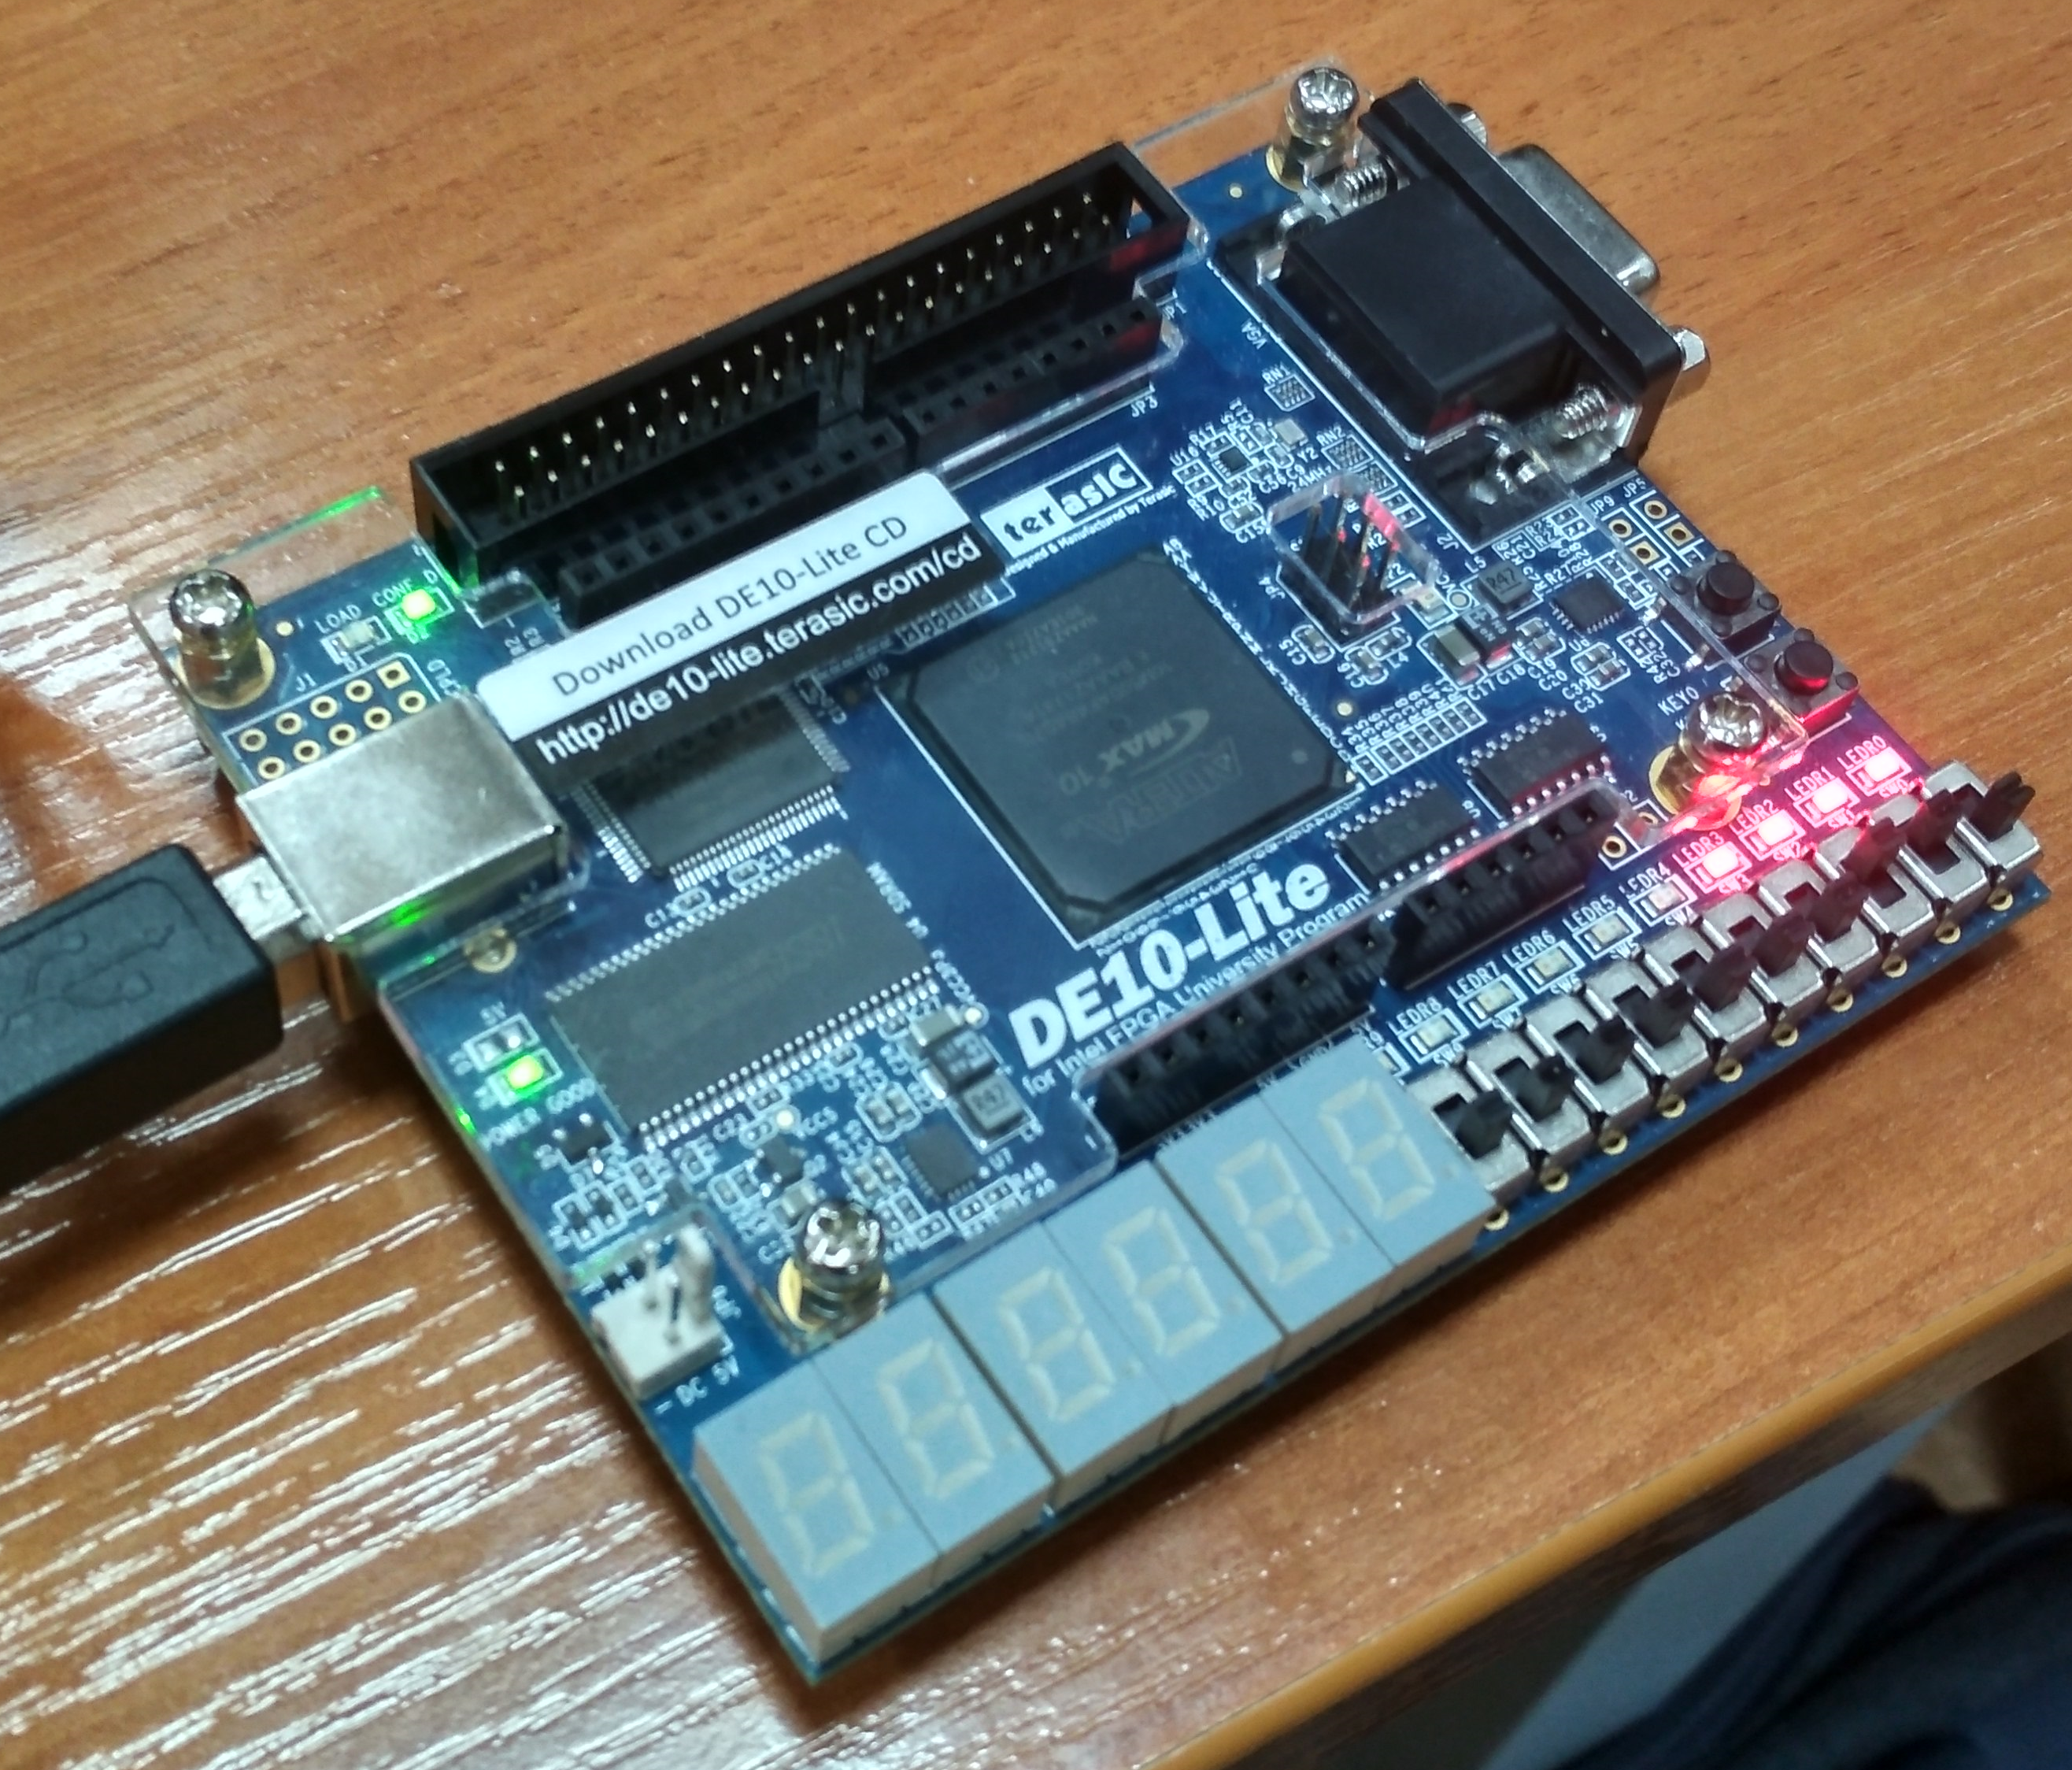
\includegraphics[width=0.7\linewidth]{image/foto2}
		\caption{Пример работающей платы}
		\label{fig:foto2}
	\end{figure}
	
	
\end{enumerate}
 
\section{Вывод}
В ходе проделанной работы были получены логические формулы СКНФ и СДНФ в минимизированном и не минимизированном видах.
Оценены аппаратные ресурсы (минимизированные схемы требуют меньшее число логических элементов) и временные ресурсы.
Получен опыт работы с $TimeQuest Timing Analyzer$.
Построена временная диаграмма для полученных функций, а также логические функции были протестированы на плате.


\newpage 
\renewcommand{\refname}{{\normalsize СПИСОК ИСПОЛЬЗОВАННЫХ ИСТОЧНИКОВ}} 
\centering 
\begin{thebibliography}{9} 
	\addcontentsline{toc}{section}{\refname} 
	\bibitem{sql} Vijayakumar P., Vijayalakshmi V., Zayaraz G. Comparative study of hyperelliptic curve cryptosystem over prime field and its survey //International Journal of Hybrid Information Technology. – 2014. – Т. 7. – №. 1. – С. 137-146.
	\bibitem{sql} Антонов А., Филиппов А., Золотухо Р. Средства системной отладки САПР Quartus II //Компоненты и технологии. – 2008. – №. 89.
\end{thebibliography}

\end{document} % конец документа